
{\bf \Huge Research Plan} \\[0.5cm]

\noindent\makebox[\linewidth]{\rule{\textwidth}{1pt}} \\

  \begin{tabular}{| l | l |}
    \hline
    Title of the project & \\ \hline
    Responsible people & Marte Løge, Lillian Røstad, Per Thorsheim\\ \hline
    Time period for the project & \\ \hline
    Amount of resources & \\ \hline
    Web address for the project & \\ \hline
  \end{tabular}

  \section*{Change Log}

    \begin{tabular}{| l | l | l | l |}
    \hline
      {\bf Version} & {\bf Date of change} & {\bf What is changed?} & {\bf Reason for change} \\ \hline
       & & &  \\ \hline
    \end{tabular}

  \section*{Research Introduction}

  My research are divided into two phases, e.g reseach project and master thesis. This research plan will cover my research in my Research project and my master thesis. My Research project will include a state-of-the-art study as well as a design of my experiment that will be conducted in my master thesis. 
  My master thesis will include data collection through the designed experiment from my research project, and a analysis of the collected data from the experiment. 

  \begin{figure}[H]
    \centering
    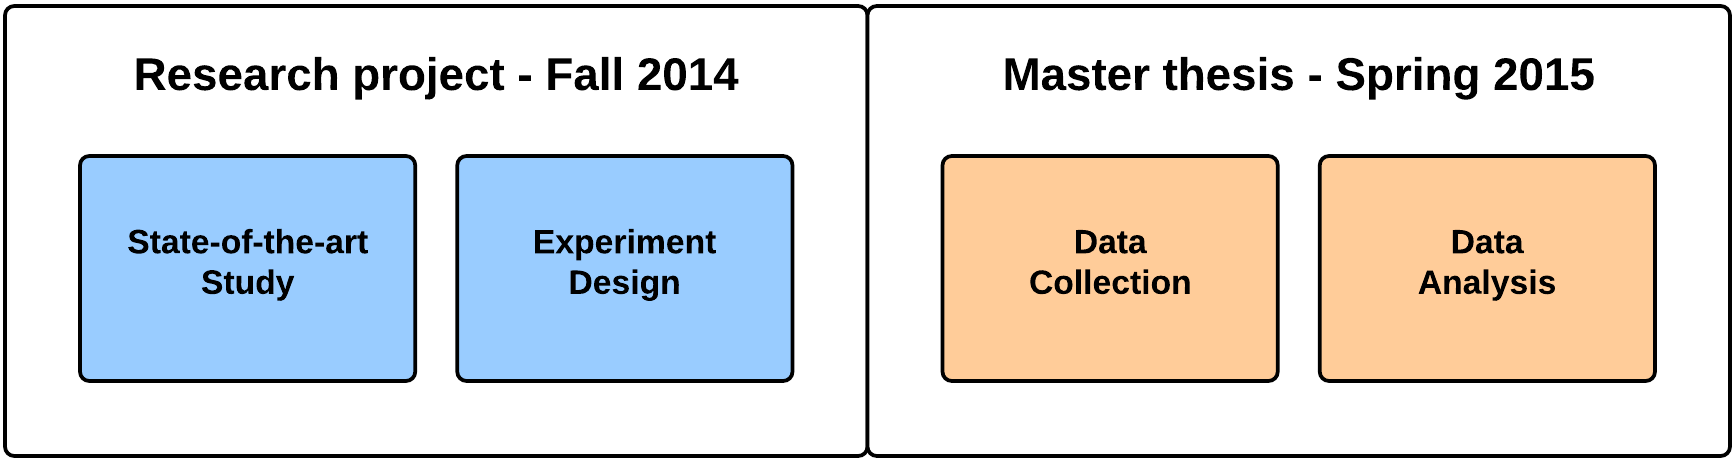
\includegraphics[width=\textwidth]{ResearchPlan1.png}
  \end{figure}

  \clearpage

  \section*{Background}
    In todays society we're addicted to our mobile devices in our every day life. Mobile devices are not just a communication tool for calling and texting, but also an important tool for every day tasks like doing our work, reading mail, pay our bills and keeping up with our social life. Our whole life is contained in one device! When such a small device is so imortant, it makes it vurnerable. How do we secure it?

    The interest in graphical passwords started by the assumption that pictures are easier to remember and more secure than words and numbers. Google's Android platform released the  functionality for Unlock Unlock Patterns in 2008. The Android Unlock pattern is a graphical password schemes that asks the user to make a pattern on a 3x3 grid by making a patten of connected nodes. Since its relese there have been a lot of discussion of its security, but few researchers have done a scientific reseach on the Android Unlock Pattern. The problem is not just the theoretical password space, but the password space in practice.

    In 2013 a research group conducted the first large-scale user study on Android Unlock Patterns. %\cite{Uellenbeck} 
    The outcome of the research was a analysis of 2900 collected Android Unlock Patterns. They found a lot of bias in the pattern making process cocluding that the schemes are less secure than its theoretical security.

    Passwords are human-chosen secrets that are connected to you as a person. When the password are created you might create a password that are a association to something you know or recognice; passwords are more than just words and numbers. The human brain interpret visual elements in a different way than numbers and words. It is important to study the bias introduced in the password making process that are introduced as a cause of human factors.

    There are conducted a lot of research that analyse human factors in PIN's and other alphanumeric passwords, but it still remains a lot of work authentication on mobile devices.

    
  
  \section*{Purpose}

  \section*{Products}

  \section*{Process}

  \section*{Participants}

  \section*{Paradigm}

  \section*{Presentation}

    \subsection*{Document}

      Both the research project and the master thesis will be delivered as a document, e.g report. 

    \subsection*{Presentation}

      The reseach project will also be a presentation at the conference P``PasswordsCon14'' in December at NTNU.


  